\documentclass{article}

\title{Optimizing fusion gain through a simplified whole-device model}

\usepackage{graphicx}
\usepackage{amsmath}
\usepackage{amssymb}
\usepackage[dvipsnames]{xcolor}
\usepackage{siunitx}
\usepackage[margin=1in]{geometry}
\usepackage{parskip}
\usepackage{circuitikz}

\usepackage{biblatex}
\addbibresource{references.bib}

\newcommand{\jack}[1]{{\color{ForestGreen} #1}}

\begin{document}
\maketitle

\section{Introduction}

This document describes a proposed modeling problem for the summer school hackathon.
We'll first describe the physical picture and motivation, then the governing equations, and finally
the configuration of software components we'll use to investigate it.

The setting is the on-axis plasma in a Z Pinch device, bounded on one end by a cathode and on the
other by an anode.
As the Z Pinch current ramps up, and the plasma undergoes compression, on-axis current must connect
through a Langmuir sheath at both electrodes.
The dynamics of the current can be modeled as a series RLC circuit--a circuit containing a resistor,
an inductor, and a capacitor.
The RLC circuit equations let us relate the plasma current, which can be observed from the solution
of our plasma kinetic or fluid equations, to the plasma voltage gap; that is, the voltage gap
across the plasma-facing electrodes.

The final piece of the picture is adiabatic compression. To a first approximation, we can assume
that the pinch is compressing adiabatically, which gives scaling relations between the plasma current
and the on-axis bulk plasma quantities, such as number density and temperature.

Putting all of these pieces together, there is a potential optimization problem to be investigated:
what combination of circuit and plasma parameters maximizes a quantity of interest such as time-integrated
neutron yield, or perhaps Q-scientific?
If the circuit model, bulk plasma model, and sheath model can all be implemented in a differentiable
program, then the optimization problem can be tackled with a derivative-based optimizer.

\begin{figure}
    \centering
    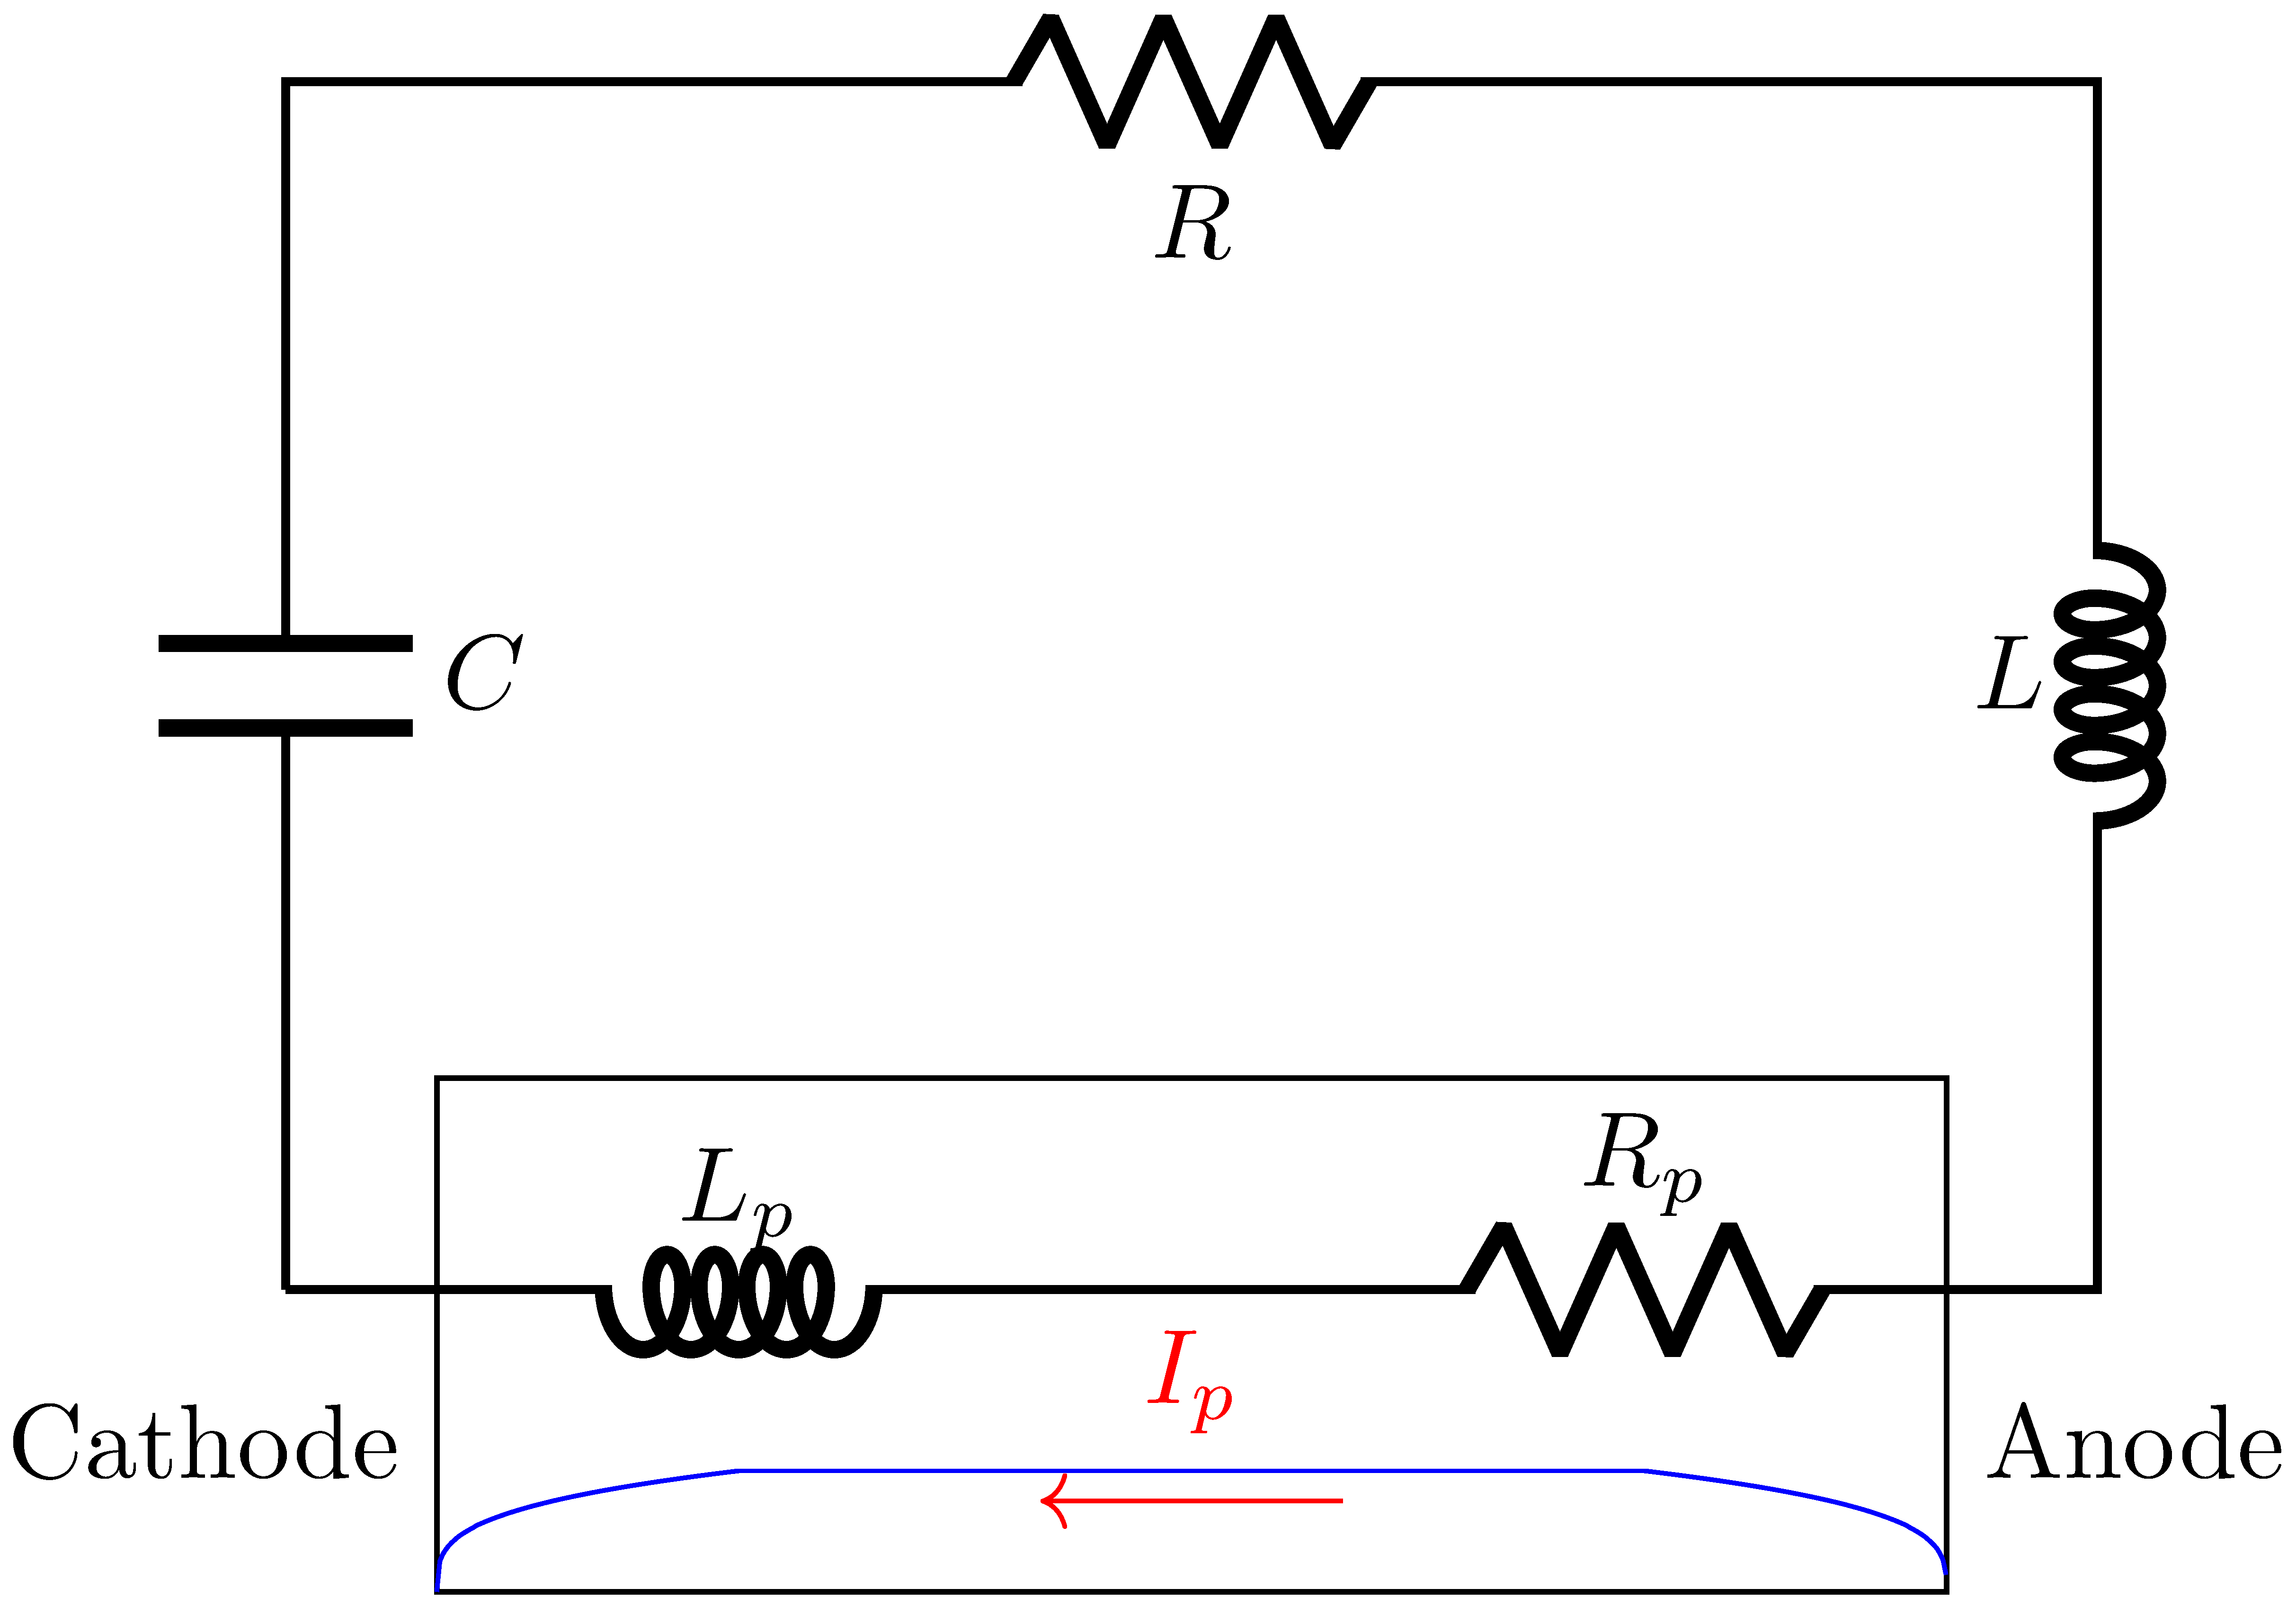
\includegraphics[width=0.6\textwidth]{images/circuit_diagram.pdf}
\end{figure}

\section{Fluid equations for an adiabatically compressing Z pinch}

%The following scaling relations hold for a Z pinch compressing adiabatically from state 1 to state 2 \cite{shumlakShearedFlowStabilizedZPinch2012} with adiabatic index $\gamma = 5/3$.

The continuity equation gives us 


\section{Circuit model}

Series RLC circuit equations for a discharging capacitor.
Let $Q$ be the charge in the capacitor, $C$ the capacitance, $R$ the resistance,
and $L$ the inductance of the circuit.
The circuit current is $I = I_p = \dot{Q}$, the rate of change of the charge.
The voltages of each component are related by
\begin{align}
V_R + V_L + V_C + V_p = 0,
\end{align}
where $V_p$ is the voltage drop across the plasma, and $V_R, V_L, V_C$ are the voltage drops across the resistor, inductor, and capacitor respectively.
From the definition of capacitance we have $V_C = Q/C$. From Ohm's law we have $V_R = IR = \dot{Q} R$, 
and $V_L = \dot{I} L = \ddot{Q} L$.

Solving for the plasma voltage gap, we get
\begin{align*}
V_p = -IR - L \frac{dI}{dt} - C \int_0^t I(\tau) \, \mathrm{d} \tau
\end{align*}

\begin{align*}
    V_{Rp} + V_{Lp} &= -V_R - V_L - V_C \\
    V_{Rp} &= -IR - L \frac{dI}{dt} - L_p \frac{dI}{dt} - C \int_0^t I(\tau) \, \mathrm{d} \tau
\end{align*}

\end{document}
